\documentclass[polish,12pt]{aghthesis}
\usepackage[utf8x]{inputenc}
\usepackage{url}
\usepackage{graphicx}
\usepackage{hyperref}
\usepackage{minted}

\graphicspath{ {./images/} }

\author{Piotr Szczygieł}

\titlePL{Gra typu Capture-The-Flag\\ oparta o reverse engineering}
\titleEN{Capture-The-Flag game based on reverse engineering}

\fieldofstudy{Informatyka}

\supervisor{dr inż.\ Łukasz Faber}

\date{\the\year}

\begin{document}

\maketitle

\tableofcontents
\newpage

\section{\SectionTitleProjectVision}
\label{sec:cel-wizja}

\subsection{Wprowadzenie}

Gra typu Capture-the-Flag jest to rodzaj zawodów z ogólnie pojętego
bezpieczeństwa komputerowego. Ich celem zwykle jest edukacja uczestników
o zabezpieczeniach systemów oraz możliwość pokazania im jak reagować
na wypadek wystąpienia rzeczywistych ataków. Zawody takie podzielone są zazwyczaj
na poszczególne zadania z różnych kategorii. Aby rozwiązać takie zadanie należy
znaleźć "flagę", którą następnie podaje się w interfejsie udostępnionym przez
organizatora zawodów. Flagą w tym wypadku jest ciąg znaków, który możemy uzyskać
poprzez rozwiązanie zadania. Przykładowo w najprostszych zadaniach
z dziedziny eksploitacji stron internetowych, flagę możemy znaleźć klikając
"Pokaż źródło strony" w przeglądarce internetowej.

\begin{figure}[ht]
    \centering
    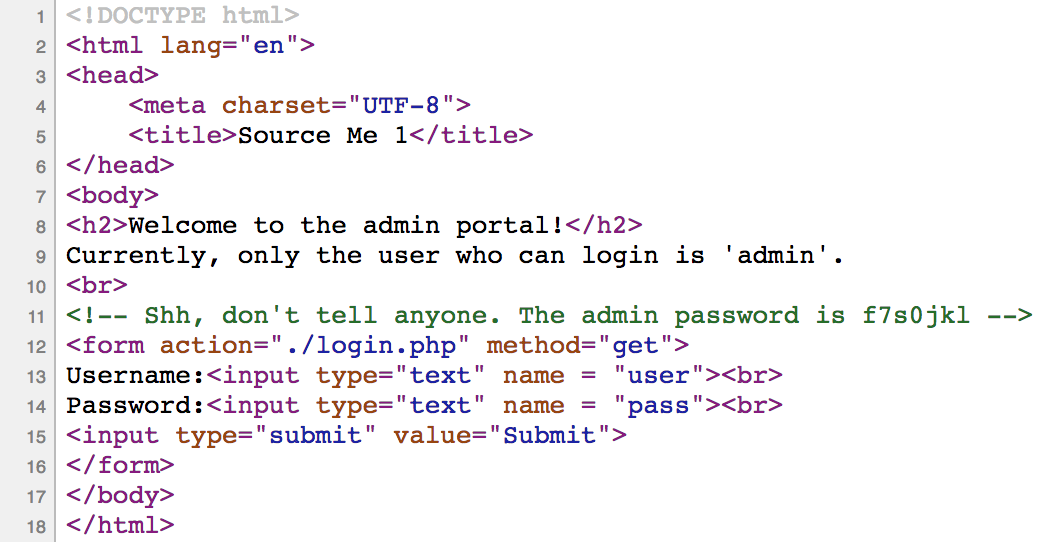
\includegraphics[width=10cm]{flag_page_source}
    \caption{Flaga \textbf{f7s0jkl} ukryta w źródle strony internetowej}
    \label{fig:flag_page_source}
\end{figure}

W tej pracy zaprezentowana będzie jednak grę oparta
wyłącznie o Reverse Engineering (ang. Inżynieria Wsteczna).
Inżynieria wsteczna oprogramowania może odbywać się na różne sposoby.
Może to być przykładowo wykorzystanie tzw. snifferów do analizy protokołów
komunikacyjnych aplikacji internetowej. W tym wypadku będzie ona jednak
zazwyczaj oznaczała proces analizy programu, aby zrozumieć co robi
oraz w jaki sposób. Przedstawione zadania można by też podpiąć do kategorii
eksploitacji binarnej (ang. Binary Exploitation), która w pewny sposób pokrywa
się z zagadnieniami Reverse Engineeringu. Jest to mianowicie proces
wykorzystywania niedoskonałości programów w celu zmuszenia ich do zrobienia
czegoś, czego w normalnej sytuacji nie powinny robić. Te dwie kategorie pokrywają
się ze sobą, ponieważ zazwyczaj nie jest możliwe rozwiązanie zadania z kategorii
eksploitacji binarnej, bez wykorzystania do tego inżynierii wstecznej. \pagebreak

Produktem końcowym będzie zbiór kilku zadań udostępniony na platformie webowej.
Platforma sama w sobie nie jest niczym specjalnym, udostępnia jedynie takie powszechne
funkcjonalności jak rejestracja użytkowników, ranking najlepszych graczy,
pobieranie zadań oraz interfejs umożliwiający wprowadzanie znalezionych
flag. Z tego względu użyta zostanie gotowa platforma CTFd \cite{CTFd}.
Użycie takiego gotowego rozwiązania pozwoli w pełni skupić się na samych zadaniach,
a ominąć takie kwestie jak np. gracze łamiący zabezpieczenia platformy.

\begin{figure}[ht]
    \centering
    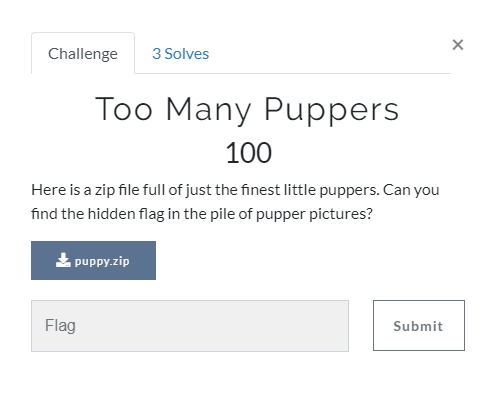
\includegraphics[width=10cm]{ctfd}
    \caption{Przykładowe zadanie na stronie demonstracyjnej CTFd}
    \label{fig:ctfd}
\end{figure}

W tej pracy opisany zostanie zarówno proces tworzenia poszczególnych zadań,
jak i przykładowe ich rozwiązania. Użyte zostało słowo "przykładowe", ponieważ
w takiej kategorii jak Binary Exploitation / Reverse Engineering liczba sposobów
na rozwiązanie danego zadania jest ograniczona jedynie przez wyobraźnie uczestnika.
Nie ograniczymy się również do korzystania ciągle z tych samych narzędzi.
Pokazane zostaną różnorodne podejścia do analizy i rozwiązywania wyzwań.
Zadania będą tworzone z zamiarem zachowania rosnącego stopnia trudności.
Na początku uczestnik będzie miał szansę rozwiązać proste zadania,
zachęcające go do dalszej rozgrywki. Finalne zadania powinny stanowić wyzwanie
nawet dla doświadczonych graczy. \pagebreak

\subsection{Dostępne platformy}

Aktualnie istnieje wiele różnych zawodów CTF online.
Jednym z popularniejszych jest \newline picoCTF \cite{picoCTF}.
Można tam wejść kiedykolwiek, zalogować się i zająć się rozwiązywaniem problemów.

\begin{figure}[ht]
    \centering
    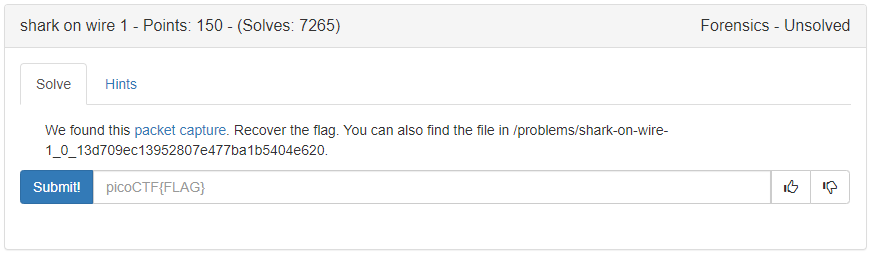
\includegraphics[width=15cm]{picoctf}
    \caption{Zadanie z kategorii Forensics na stronie picoCTF}
    \label{fig:picoctf}
\end{figure}

Główną motywacją do napisania tej pracy jest fakt, że strony tego typu często skupiają
się na zadaniach w takich kategoriach jak Forensics czy Web Exploitation.
Mnie natomiast bardzo interesuję temat inżynierii wstecznej i chciałem
przygotować wyzwania oparte o zadania tylko z tej kategorii.

\subsection{Języki programowania i narzędzia}

Zadania będą tworzone w języku C. Jest to powszechnie znany język, który
z wyłączoną zbyt agresywną optymalizacją ze strony kompilatora, generuje
w miarę przewidywalny kod maszynowy. Zaletą tego jest to, że narzędzia
do debugowania, dezasemblacji oraz wykonywania innych analiz programów
dobrze radzą sobie z takimi plikami. Dzięki temu język ten
zapewni nam kontrolę nad tym w jakim stopniu graczowi ułatwimy
lub utrudnimy rozgrywkę. W celu zapewnienia większej różnorodności
środowisk korzystać będziemy zarówno z systemu Windows jak i Linux.

Do rozwiązywania zadań posłużymy się różnorodnymi rodzajami narzędzi.
Poczynając od linuxowych programów linii poleceń takich jak \emph{strings}
czy \emph{gdb}, pisania własnych narzędzi w języku \emph{Python},
czy w końcu korzystając z pełnoprawnych narzędzi z interfejsem graficznym takich
jak używana przez NSA \emph{Ghidra}, \emph{Cutter}, czy debugger dla systemu
Windows \emph{RemedyBG}.

\clearpage

\section{\SectionTitleScope}
\label{sec:zakres-funkcjonalnosci}

\subsection{Platforma}

Do interfejsu webowego skorzystamy z gotowej platformy CTFd \cite{CTFd}.
Finalny produkt będzie dostępny pod adresem
\href{https://ctf.szczygiel.dev}{https://ctf.szczygiel.dev}.
Strona postawiona będzie na prywatnym serwerze VPS. Platforma będzie
uruchomiona w środowisku docker \cite{docker},
a wystawiona do świata będzie poprzez serwer Caddy \cite{Caddy},
który w prosty sposób zapewni nam HTTPS, dzięki organizacji Let's Encrypt \cite{lets_encrypt}.

\subsection{Użytkownicy}

Użytkownikiem systemu będzie każda osoba zainteresowana rozwiązywaniem
tego rodzaju zadań. Może to być zarówno ktoś kształcący się lub pracujący
w dziale informatycznym, jak i osoba dla której jest to jedynie hobby.

Wszystkie gotowe zadania zostaną wrzucone na platformę, dzięki czemu
każda zainteresowana osoba będzie mogła spróbować swoich sił.

\clearpage

\subsection{Prezentacja interfejsu użytkownika}

\begin{figure}[ht]
    Pierwsze co zobaczy każdy użytkownik wchodzący na platformę, to strona główna.
    Będzie z niej można przejść do reszty podstron, takich jak logowanie, rejestracja,
    wylogowanie, spis graczy, tabela wyników oraz lista dostępnych zadań.

    \vspace{1cm}

    \centering
    
\includegraphics[width=14cm]{szczygiel_dev}
    \caption{Strona głowna platformy CTF}
    \label{fig:szczygiel_dev}
\end{figure}

\begin{figure}[ht]
    Poniżej przedstawiony jest interfejs rejestracji nowego użytkownika.
    Nie będzie to nic skomplikowanego - wystarczy podać login, email oraz hasło.

    \vspace{1cm}

    \centering
    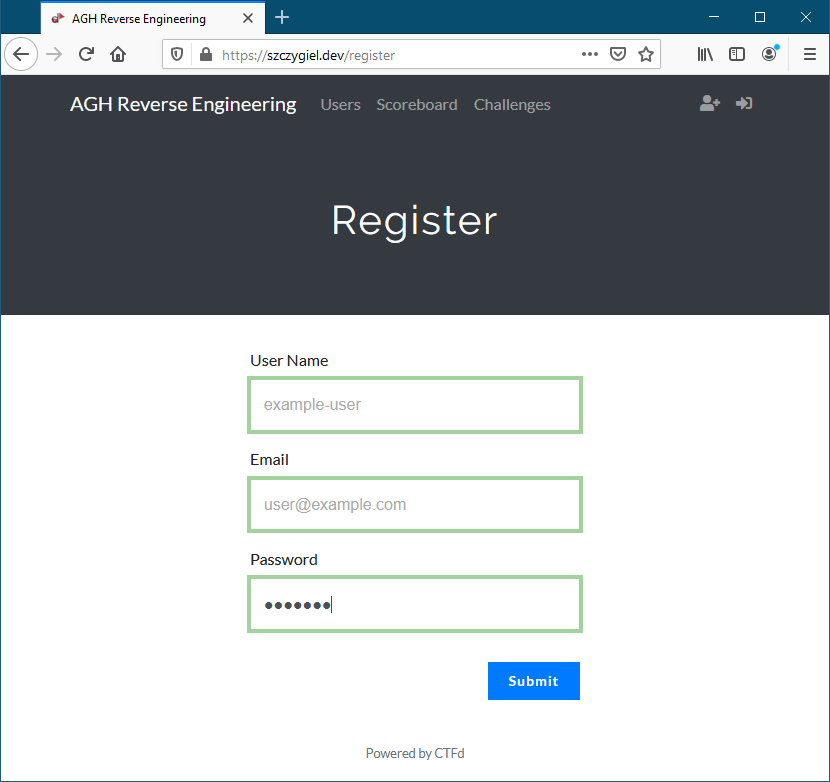
\includegraphics[width=14cm]{szczygiel_dev_register}
    \caption{Rejestracja nowego użytkownika}
    \label{fig:szczygiel_dev_register}
\end{figure}

\begin{figure}[ht]
    Jeśli użytkownik posiada konto to będzie się mógł na nie zalogować.

    \vspace{1cm}

    \centering
    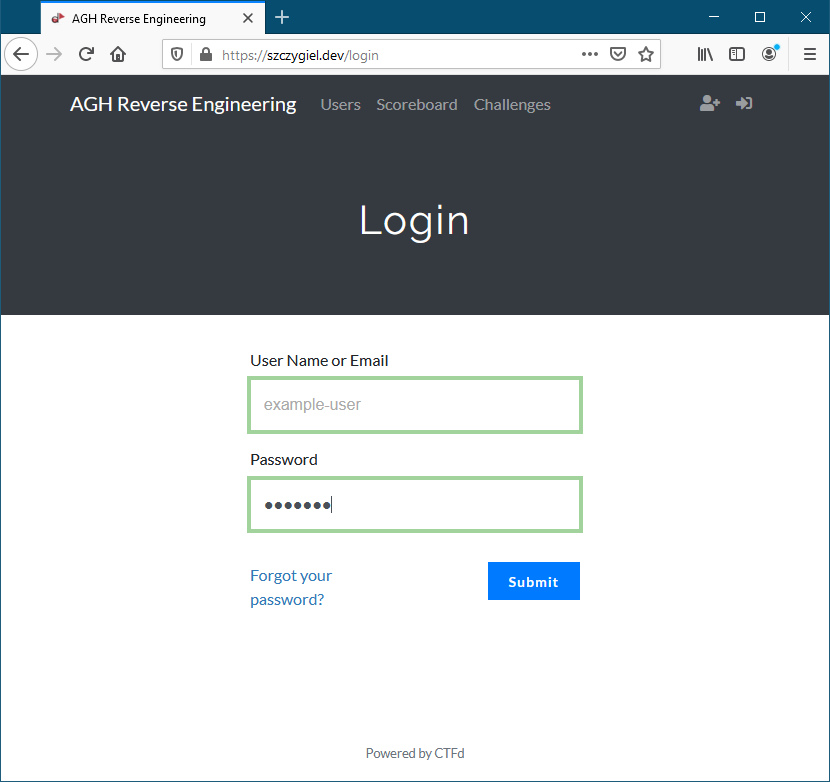
\includegraphics[width=14cm]{szczygiel_dev_login}
    \caption{Panel logowania dla istniejącego użytkownika}
    \label{fig:szczygiel_dev_login}
\end{figure}

\begin{figure}[ht]
    Będąc zalogowanym, można wybrać zadanie które ma się ochote rozwiązać.

    \vspace{1cm}

    \centering
    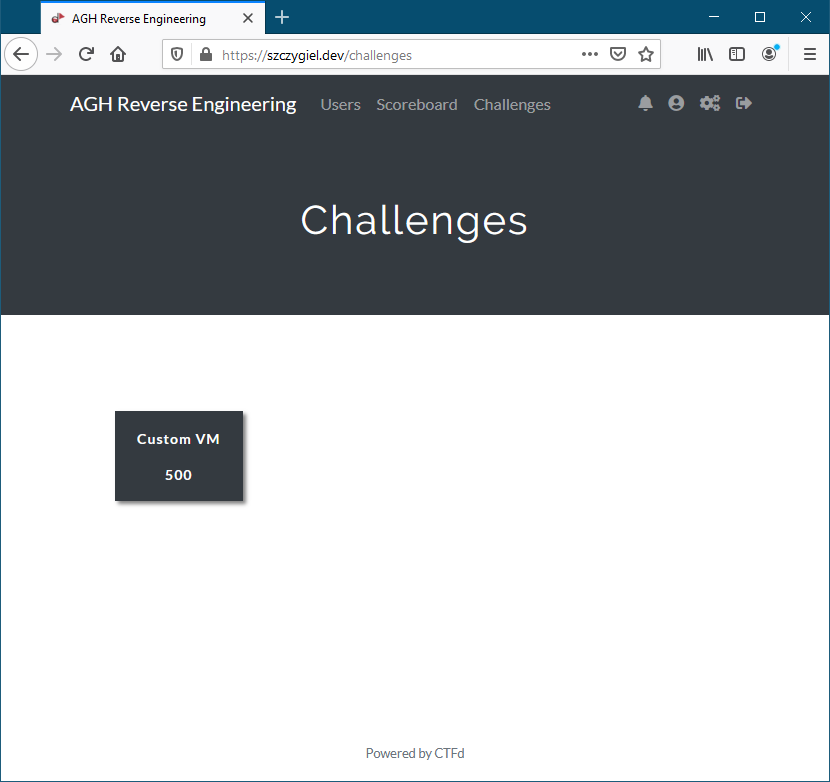
\includegraphics[width=14cm]{szczygiel_dev_challenges}
    \caption{Wybór zadania do rozwiązania}
    \label{fig:szczygiel_dev_challenges}
\end{figure}

\begin{figure}[ht]
Po wybraniu interesującego nas zadania, można pobrać dostarczony plik,
    a następnie po rozwiązaniu zadania wprowadzić prawidłową (lub nie) flagę.

    \vspace{1cm}

    \centering
    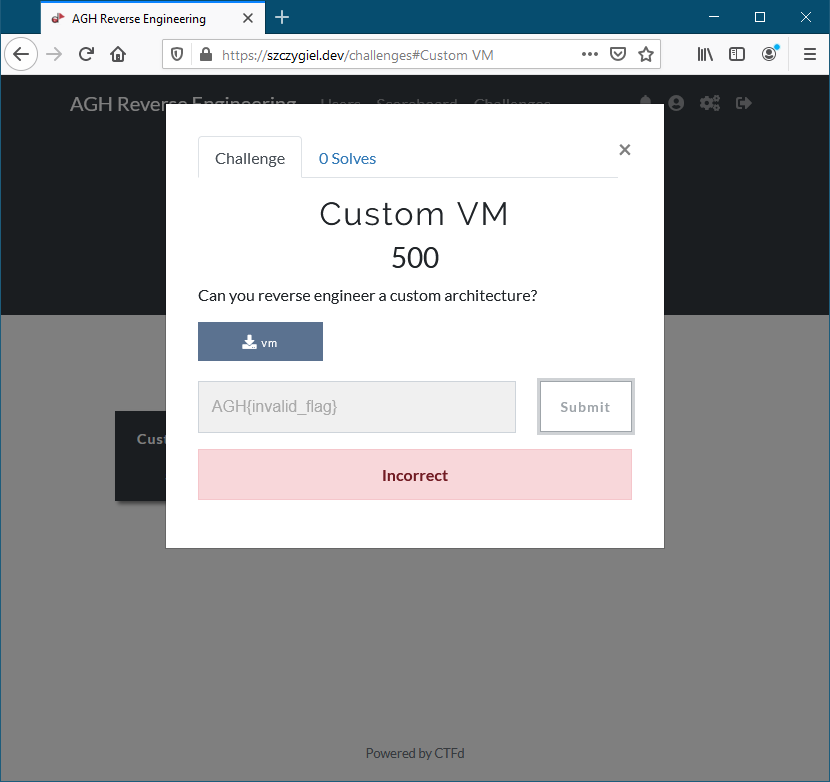
\includegraphics[width=14cm]{szczygiel_dev_incorrect}
    \caption{Interfejs zadania oraz wprowadzenie nieprawidłowej flagi}
    \label{fig:szczygiel_dev_incorrect}
\end{figure}

\begin{figure}[ht]
    Po wprowadzeniu prawidłowej flagi otrzymamy stosowny komunikat.
    Można również zauważyć, że zadanie w tle zmieniło kolor na zielony.

    \vspace{1cm}

    \centering
    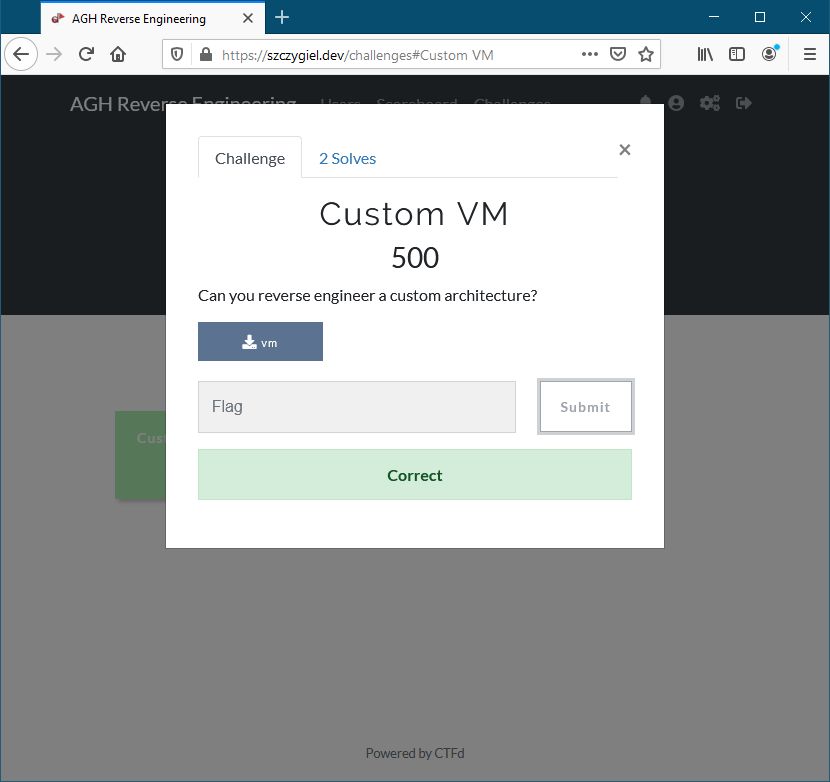
\includegraphics[width=14cm]{szczygiel_dev_correct}
    \caption{Efekt wprowadzenia prawidłowej flagi}
    \label{fig:szczygiel_dev_correct}
\end{figure}

\begin{figure}[ht]
    Dostępna jest również lista zarejestrowanych użytkowników.
    Można wejść w profil każdego użytkownika i zobaczyć jego postępy.

    \vspace{1cm}

    \centering
    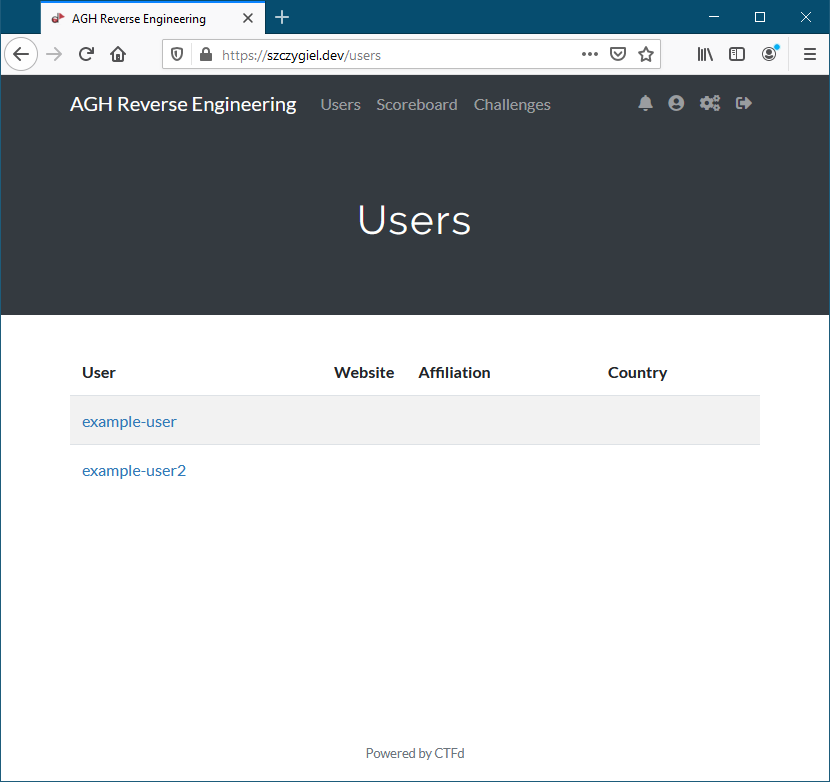
\includegraphics[width=14cm]{szczygiel_dev_users}
    \caption{Spis zarejestrowanych użytkowników}
    \label{fig:szczygiel_dev_users}
\end{figure}

\begin{figure}[ht]
Wchodząc na profil użytkownika można zobaczyć o nim różne informacje.
Jest to przede wszystkim rozkład prawidłowych oraz nieprawidłowych
    wprowadzeń flag oraz wykres posiadanych punktów w czasie.
    Na dole widzimy również wszystkie rozwiązane przez użytkownika zadania.

    \vspace{1cm}

    \centering
    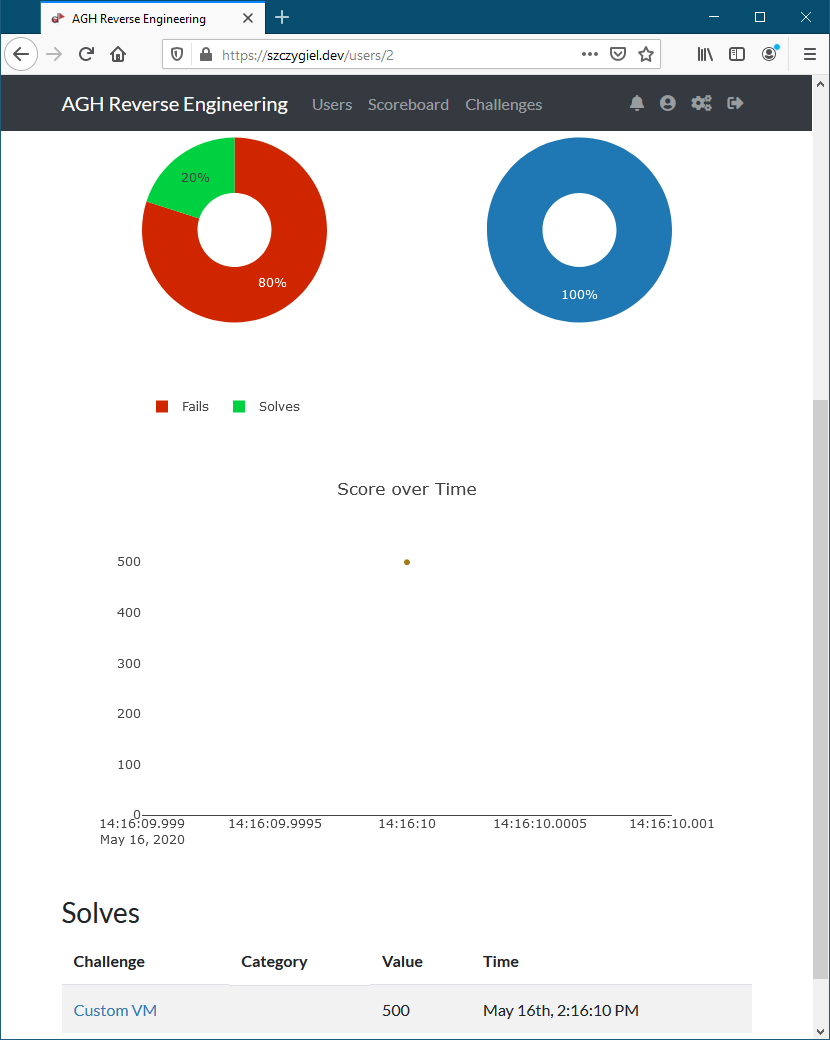
\includegraphics[width=14cm]{szczygiel_dev_user_info}
    \caption{Szczegóły postępów konkretnego użytkownika}
    \label{fig:szczygiel_dev_user_info}
\end{figure}

\begin{figure}[ht]
    Każdy użytkownik może również zmienić oraz dodać informację o sobie.
    Będzie mógł zmienić nazwę użytkownika, email, hasło, oraz dodać
    takie szczegóły jak strona internetowa, firma dla której pracuję czy kraj pochodzenia.

    \vspace{1cm}

    \centering
    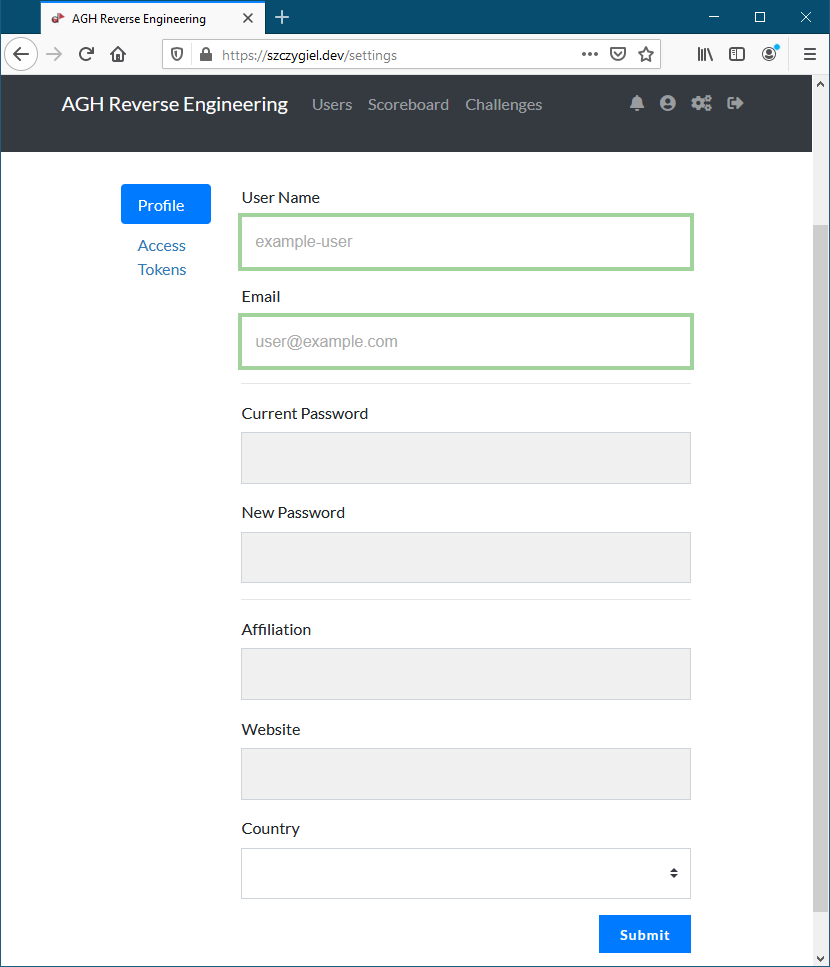
\includegraphics[width=14cm]{szczygiel_dev_settings}
    \caption{Edycja profilu użytkownika}
    \label{fig:szczygiel_dev_settings}
\end{figure}

\clearpage

\section{\SectionTitleRealizationAspects}
\label{sec:wybrane-aspekty-realizacji}

\subsection{100-simple}

\subsection{200-game}

\subsection{300-strcmp}

\subsection{400-decrypt}

\subsection{500-secret-shell}

\subsection{600-custom-vm}

\clearpage

\section{\SectionTitleWorkOrganization}
\label{sec:organizacja-pracy}
\emph{Struktura zespołu (role poszczególnych osób), krótki opis i
    uzasadnienie przyjętej metodyki i/lub kolejności prac, planowane i
    zrealizowane etapy prac ze wskazaniem udziału poszczególnych
    członków zespołu, wykorzystane praktyki i narzędzia w zarządzaniu
    projektem.}

\clearpage

\section{\SectionTitleResults}
\label{sec:wyniki-projektu}

\subsection{100-simple}

\subsection{200-game}

\subsection{300-strcmp}

\subsection{400-decrypt}

\subsection{500-secret-shell}

\subsection{600-custom-vm}

\clearpage

\bibliography{bibliography}

\end{document}
